%!TEX root = origin_elements_lecture_notes.tex

\chapter{Big Bang Nucleosynthesis}

In order to understand primordial / \acf{bbn}, we need to first look at some fundamental observations that define cosmology. In addition, we also need to introduce the standard model of cosmology. Note that this is only a very brief introduction into a topic that could be a whole course by itself.

\section{Fundamental Cosmological Observations}

\subsection{Olbers' paradox}

One of the most fundamental observations that goes back to Kepler (1610), Halley (1721), de Cheseaux (1744), and is today known as Olbers' (1823) paradox is the fact that the night sky is dark. If one assumes an infinite, homogeneous space filled with stars, this space would appear infinitely bright to the observer on Earth. The apparent luminosity of a star can be described as
\begin{equation}\label{eqn:bbn:relative_luminosity}
    l = \frac{L}{4 \pi r^{2}} \propto r^{-2},
\end{equation}
where $L$ is the star's luminosity and $r$ its distance from Earth. Assuming a density of stars $n$, a spherical shell of thickness $dr$ at distance $r$ from Earth would contain
\begin{equation}
    dN = 4 \pi n r^2 dr \propto r^2
\end{equation}
stars. The total energy density of all stars for an observer can thus be calculated as
\begin{equation}\label{eqn:bbn:total_energy_density}
    \varepsilon_s = \int_0^{\infty} \frac{L}{4\pi r^2} dN = nL \int_{0}^{\infty} dr.
\end{equation}
In contrast to our experience this integral is divergent, thus the night sky should be infinitely bright. 

This paradox cannot be simply solved by assuming absorption of light in the interstellar medium, e.g., by dust. The energy from all stars would over time heat up this dust until it radiates as bright as the stars themselves. One factor that slightly helps is that stars will overlap with each other. You can picture this scenario however like standing in a dense forest where, as far as you can see, every line of sites terminates in a tree trunk. For the universe this would mean that every line of sight will terminate at the surface of a star. Stars cover each other, so the night sky would not seem infinitely bright but homogeneously about as bright as the Sun. This still does not agree with our experience.

The solution to the paradox lies in the fact that the universe is expanding. The wavelength of the light that arrives expands along with the universe and is thus shifted to the red (Doppler shift). The result is that the relative luminosity, as given in equation \eqref{eqn:bbn:relative_luminosity}, is in fact $l\propto r^{-3}$. Plugging this into equation~\eqref{eqn:bbn:relative_luminosity} results in the integral converging. In addition, there the universe has a horizon at distance
\begin{equation}
    R \simeq ct.
\end{equation}
Here, $c$ is the speed of light and $t$ the approximate age of the universe. The visible part of space and thus the energy density become finite.

\infobox{Doppler effect}{Let us assume that a source emits an electromagnetic wave with wavelength $\lambda_s$. An observer that moves with a velocity $\vec{v}$ with respect to that source will register a shifted frequency $\lambda_r$. For light, and considering special relativity, this effect will result in a blueshift if the observer moves towards the source and in a redshift if the observer moves away from the source. For two objects that move directly towards or away from each other, the relativistic Doppler shift for light can be written as
\begin{equation}\label{eqn:bbn:relativistic_doppler_shift}
    \lambda_r = \sqrt{\frac{1+\beta}{1-\beta}} \lambda_s,
\end{equation}
where $\beta = v/c$, i.e., the speed of the observer $v$ with respect to the speed of light $c$. Sources moving away from each other hereby have a postive velocity ($\beta > 0$), sources moving towards each other a negative one ($\beta < 0$).}

\subsection{Hubble's Law}

\begin{figure}[tb]
    \centering
    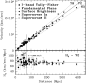
\includegraphics[width=0.5\textwidth]{graphics/bbn/hubble_diagram}
    \caption{Hubble diagram of velocity (top) and value of $H_0$ (bottom) as a function of distance. \cite{freedman01}, \copyright\ 2001 The American Astronomical Society.} 
    \label{fig:bbn:hubble_diagram}
\end{figure}
The expansion of the universe can in fact be observed. Figure~\ref{fig:bbn:hubble_diagram} shows the Hubble diagram for many observations, taken from \citet{freedman01}. The diagram on top shows the velocity of objects relative to Earth as a function of their distance. Using the Doppler shift one can see that the velocity, which is away from the observer in this case, is proportional to the redshift of the object. Here, the distance is given in megaparsec, where 1\,\ac{pc} is approximately 3.26 light years. The linear relationship between velocity and distance (R) can be written as
\begin{equation}
    \left(\frac{\dot{R}}{R}\right)_0 = H_0 = \mathrm{constant}.
\end{equation}
The subscript zero hereby describes the present-day value of the constant. The constant $H_0$ is commonly called the Hubble constant and its value is about $H_0 = 70\,\mathrm{km}\,\mathrm{s}^{-1}\,\mathrm{Mpc}^{-1}$. Note that the Hubble constant is given in units of one over seconds. The reciprocal value of the $H_0$ thus defines a time, the so-called Hubble time. If the expansion of the universe is never accelerated, its age could be determined as
\begin{equation}
    t_0 \leq \frac{1}{H_0} = 1.4 \times 10^{10}\,\mathrm{a}.
\end{equation}

The distance of a galaxy is often expressed by its redshift. Let $\lambda$ be the wavelength sent out from the galaxy in question and $\lambda_0$ the wavelength received today. The redshift $z$ can then be written as
\begin{equation}\label{eqn:bbn:redshift}
    1+z = \frac{\lambda_0}{\lambda} = \frac{R_0}{R}.
\end{equation}
Here, $R$ is introduced as the so-called scale factor of the universe.

Since the universe consists of mass that interacts gravitationally with each other, we can define a deceleration parameter $q_0$ for the universe such that
\begin{equation}
    \label{eqn:bbn:decceleration}
    q_0 \equiv -\left(\frac{\ddot{R} R}{\dot{R}^2}\right) = - \frac{\ddot{R_0}}{R_0 H_0^2}.
\end{equation}


\subsection{Density of Matter}
By density one generally refers to the total energy density of all components (radiation, matter, and dark energy) divided by $c^2$. While radiation dominated in the early universe, matter or even dark energy dominates today. The total density of matter in the universe can be measured by determining the total mass of individual galaxies. An estimated density can thus be given as
\begin{equation}
    2 \times 10^{-31}\,\mathrm{g}\,\mathrm{cm}^{-2} \leq \rho_0 \leq 2\times10^{-30}\,\mathrm{g}\,\mathrm{cm}^{-2}.
\end{equation}

\morebox{Dark matter}{In 1933, Fritz Zwicky noticed that galactic cluster do not rotate as expected. By constraining the observed mass in the cluster and observing its rotation, Zwicky noticed that some matter was missing. He called this dark matter. Figure~\ref{fig:bbn:galactic_rotation} shows an example of the expected and observed rotation curves. From this and further observations we can derive that dark matter makes up around 85\% of all matter in the universe. Only 15\% of the matter in the universe consists of baryons, e.g., particles made up of quarks such as neutrons and protons.}
\begin{figure}[tb]
    \centering
    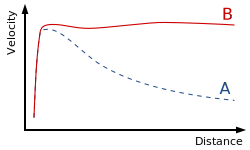
\includegraphics[width=0.45\textwidth]{graphics/bbn/galactic_rotation}
    \caption{Galactic rotation: Case A shows the expected behavior, case B the observed one. Credit: \href{https://en.wikipedia.org/wiki/Dark_matter}{Wikipedia}.}
    \label{fig:bbn:galactic_rotation}
\end{figure}



\subsection{Cosmic Microwave Background}

In the Big Bang model, the universe started from a very hot and dense state. One expected remnant of this state is a relic radiation that in fact was detected in 1965 by Arno Penzias and Robert Wilson \citep{penzias65}. The detection of this \ac{cmb} is one of the pillars supporting the Big Bang model to describe the origin of the universe. The origin of the \ac{cmb} will be discussed in further detail below.

The \ac{cmb} is a thermal blackbody radiation with a measured temperature of $2.72548 \pm 0.00057$\,K. The peak of this radiation is in the microwave range and cannot be observed from Earth. Space missions such as \href{https://map.gsfc.nasa.gov/}{\ac{wmap}} and \href{http://www.esa.int/Science_Exploration/Space_Science/Planck}{Planck} measured the \ac{cmb} in detail. A map of the \ac{cmb} is shown in Figure~\ref{fig:bbn:wmap_cmb}.
\begin{figure}[tb]
    \centering
    \includegraphics[width=0.75\textwidth]{graphics/bbn/wmap_cmb}
    \caption{\ac{wmap}'s image of the \ac{cmb}. Shown is averaged data from nine years of measurements. Credit: \href{https://map.gsfc.nasa.gov/media/121238/index.html}{NASA}.}
    \label{fig:bbn:wmap_cmb}
\end{figure}



\section{The Standard Model of Cosmology}

The standard model of cosmology describes the origin of the universe and its evolution based on one singular event: the Big Bang. With the Big Bang, space, time, and matter came into existence and the universe developed from its hot, dense state to the cold and transparent state we see today.

\subsection{Assumptions}\label{sec:bbn:standard_model:assumptions}

The standard model of cosmology is based on several key assumptions. Here we focus on the ones that are of importance to understand \ac{bbn}.

\begin{enumerate}
    \item The cosmological principle is valid. This states that the spatial distribution of matter in the universe in homogeneous and isotropic. \label{it:bbn:cosmological_principle}
    \item The overall charge in the universe is zero.
    \item The universe is made of matter and not of antimatter. This assumption in fact directly contradicts the cosmological principle (assumption \ref{it:bbn:cosmological_principle}) since it requires that there was an overabundance of baryons compared to antibaryons at the start of the universe, making it thus inhomogeneous. This overabundance of matter is to this date not fully explained and remains under active investigation.
    \item At temperature $T<10^{11}$\,K (approximately 10\,ms after the Big Bang), all heavy particles were annihilated and the density of the universe is defined by photons, neutrinos ($\nu$), electron and positrons ($\mathrm{e}^{\pm}$), and the remaining baryons.
\end{enumerate}


\subsection{Temperature and Density Evolution}

\begin{figure}[tb]
    \centering
    \includegraphics[width=0.6\textwidth]{graphics/bbn/wagoner67_fig1}
    \caption{The temperature and density evolution of the universe in the framework of the standard model of cosmology. Taken from \citet{wagoner67}. \copyright\ American Astronomical Society.}
    \label{fig:bbn:cosmology_phases}
\end{figure}
Figure~\ref{fig:bbn:cosmology_phases} shows the temperature and density evolution of the universe in the framework of the standard model of cosmology \citep{wagoner67}. The horizontal axis show the expansion factor $R/R_0$ as defined in equation \ref{eqn:bbn:redshift} on the bottom and the time since the Big Bang on the top. The vertical axes show the temperature (left) and the density (right). The standard model description starts at around 10\,ms with all constituents in equilibrium. \acl{bbn} sets in at a temperature of around $10^{9}$\,K. 



\section{Big Bang Nucleosynthesis}

\subsection{The Proton-to-Neutron Ratio}

In the beginning at a temperature of around $10^{11}$\,K (see Figure~\ref{fig:bbn:cosmology_phases}), the protons and neutrons are in thermodynamic equilibrium. Statistical mechanics shows that the energy of such a system can be expressed using the Boltzmann distribution for the individual states. This can be used to express the ratio of the number of protons to the number of neutrons in equilibrium conditions as
\begin{equation}\label{eqn:bbn:td_equilibrium_number_ratios}
    \left(\frac{n_\mathrm{p}}{n_\mathrm{n}}\right)_\mathrm{eq} 
        = \frac{\lambda_\mathrm{np}}{\lambda_\mathrm{pn}}
        = \exp\left(\frac{(m_\mathrm{n} - m_\mathrm{p})c^2}{kT}\right)
        = \exp\left(\frac{1.501}{T_{10}}\right).
\end{equation}
Here, $\lambda_\mathrm{np}$ and $\lambda_\mathrm{pn}$ are the reaction rates to turn a neutron into proton and vice verse, respectively. For $T\rightarrow\infty$ protons and neutrons will have equal abundances. At lower temperatures however, protons will become more abundant. 

We can rewrite equation~\eqref{eqn:bbn:td_equilibrium_number_ratios} to express the mass fractions of neutrons in equilibrium as
\begin{equation}
    X_\mathrm{n,eq} = \left(\frac{n_\mathrm{n}}{n_\mathrm{p} + n_\mathrm{n}}\right)_\mathrm{eq}
    = \frac{1}{(n_\mathrm{p} / n_\mathrm{n})_\mathrm{eq} + 1}
    = \frac{\lambda_\mathrm{pn}}{\lambda_\mathrm{pn} + \lambda_\mathrm{np}}.
\end{equation}


The nucleons react with each other via the weak force and the following reactions are possible:
\begin{eqnarray}
    \mathrm{n} + \nu &\longleftrightarrow& \mathrm{p} + \mathrm{e}^{-} \\
    \mathrm{n} + \mathrm{e}^{+} &\longleftrightarrow& \mathrm{p} + \bar{\nu} \\
    \mathrm{n} &\longrightarrow& \mathrm{p} + \mathrm{e}^{-} + \bar{\nu} \label{eqn:bbn:neutron_decay_reaction}
\end{eqnarray}
Reaction \eqref{eqn:bbn:neutron_decay_reaction} is the free decay of neutrons and has a half-life of 610\,s. This reaction can thus be neglected at the beginning since it is very long compared to all other reactions. The neutron mass fraction over time follows thus the differential equation
\begin{equation}
    \frac{d}{dt}X_\mathrm{n}(t) = -\lambda_\mathrm{np}(t)X_\mathrm{n}(t) + \lambda_\mathrm{pn}(t)[1-X_\mathrm{n}(t)].
\end{equation}
With decreasing temperature the reaction rates $\lambda_\mathrm{np}$ and $\lambda_\mathrm{pn}$ go rapidly towards zero such that after around 10\,s the proton to neutron ratio is frozen in place. Calculating reaction rate values, e.g., as in \citet{peebles66apj}, the neutron mass fraction at freezeout (when the reaction rates $\lambda_\mathrm{np}$ and $\lambda_\mathrm{pn}$ go to zero) is
\begin{equation}
    X_\mathrm{n,freeze} = 0.164.
\end{equation}
From this time on, the only reaction taking place is free neutron decay, see reaction~\eqref{eqn:bbn:neutron_decay_reaction}. Since the half-life of neutrons is fairly short, they must rapidly after the freezeout be captured as part of atomic nuclei in order to not decay away.


\subsection{Nucleosynthesis of Deuterium}

Deuterium has a mass of $m_\mathrm{D} = 1875.612928$\,MeV, while a proton and neutron have masses of $m_\mathrm{p} = 938.272088$\,MeV and $m_\mathrm{n} = 939.565421$\,MeV (see info box below for an explanation of measurements in eV).  
\begin{table}[b]  % since info boxes are in tabular environments...
\infobox{Measurements in eV}{In nuclear physics, masses are often expressed in mega electronvolts or MeV, which is technically not a mass but an energy. The mass of the particle is related to its energy via Einstein's equation $m=E/c^2$. Thus, energy and mass are directly related with $c$, the speed of light, as a proportionality constant. Similarly we can write the momentum of a particle as $\vec{p} = E \vec{c}^{-1}$ and the temperature of a system as $T = E k_B^{-1}$. Here, $k_B$ is the Boltzmann constant. Since mass, momentum, and temperature are related to energy via constants, these quantities are often expressed as energies.}
\end{table}
Deuterium, an isotope of hydrogen (\ex{2}H), consists of one proton and one neutron. However, summing the mass of one proton and one neutron results in a mass that is $\Delta m = 2.22$\,MeV larger than the mass of deuterium. This so-called mass defect defines the binding energy of deuterium and is the reason why energy is released when a proton and neutron are fused together. In chemistry this would be called an exothermic reaction. It can be written as
\begin{equation}\label{eqn:bbn:deuterium_formation_reaction}
    \mathrm{p} + \mathrm{n} \longrightarrow \mathrm{D} + \gamma.
\end{equation}
\begin{figure}[tb]
    \centering
    \includegraphics[width=0.5\textwidth]{graphics/bbn/planck_radiation_bbn}
    \caption{Spectral energy of black body radiation at the temperature when neutrons and protons are in equilibrium ($T_{9} \approx 5$) and when deuterium fusion can start ($T_{9}\approx1$). Prior to this temperature, the photon energies are too high and destroy newly formed deuterium effectively.}
    \label{fig:bbn:planck_radiation_deuterium_fusion}
\end{figure}

At the time when $n_\mathrm{p}/n_\mathrm{n}$ is frozen, the temperature of the universe is still $T\approx 5\times 10^{9}$\,K. Any deuterium that forms at this temperature is effectively destroyed right away again, since many photons have enough energy to dissociate the binding energy of 2.22\,MeV. Figure~\ref{fig:bbn:planck_radiation_deuterium_fusion} shows the spectral energy of a blackbody at this high temperature as a function of the frequency of the photons (bottom axis) and as function of their energy in MeV (top axis). The black, dashed line shows the deuterium binding energy. Note that both axes of the figure are logarithmic. Clearly, at $T_9 = 5$ many photons still have high enough energies. The universe thus first needs to cool down below $T_9 \approx 1$ before deuterium can effectively form. 

The exact temperatures, as just described, do not only depend on the temperature but also on the abundance of photons. Furthermore, the temperature is directly related to the density of the universe. Figure~\ref{fig:bbn:planck_radiation_deuterium_fusion} thus only gives a relative insight into the dissociation of deuterium. More detailed calculations can be found in the literature, e.g., in \citet{wagoner67}.

The drop in temperature of the universe from when proton and neutron abundances are frozen until deuterium can effectively form without being destroyed takes about 220\,s. During this time, the neutrons still undergo free decay. Using equation~\eqref{eqn:radioactive_decay} we can calculate that by the time deuterium fusion becomes significant, another $\sim20$\% of the neutrons decay.
This leaves behind a neutron fraction of
\begin{equation}
    X_n = 0.128
\end{equation}
at the start of \ac{bbn}.

\subsection{Nucleosynthesis of Helium}

Once deuterium has formed, more reactions can take place. Some of these reactions are:
\begin{eqnarray}
    \mathrm{D} + \mathrm{D} &\longleftrightarrow& ^3\mathrm{He} + \mathrm{n} \\
    \mathrm{T} + \mathrm{p} &\longleftrightarrow& ^3\mathrm{He} + \mathrm{n} \\
    \mathrm{T} + \mathrm{D} &\longleftrightarrow& ^4\mathrm{He} + \mathrm{n} \\
    \mathrm{p} + \mathrm{D} &\longleftrightarrow& ^3\mathrm{He} + \gamma \\
    \mathrm{n} + \mathrm{D} &\longleftrightarrow& \mathrm{T} + \gamma \\
    \mathrm{p} + \mathrm{T} &\longleftrightarrow& ^4\mathrm{He} + \gamma \\
    \mathrm{n} + {^3}\mathrm{He} &\longleftrightarrow& ^4\mathrm{He} + \gamma \\
    \mathrm{D} + \mathrm{D} &\longleftrightarrow& ^4\mathrm{He} + \gamma
\end{eqnarray}
Here, T is a tritium nucleus, another isotope of hydrogen with two neutrons (\ex{3}H). The reaction rates for these individual paths can be calculated, however, let us first estimate the dominant product of big bang nucleosynthesis. For deuterium above we determined a binding energy of 2.22\,MeV. Calculating the mass defect and thus the binding energy for \ex{3}He and \ex{4}He gives 6.70\,MeV and 27.3\,MeV, respectively. A better way to compare these binding energies is however to determine the binding energy per nucleon. For \ex{3}He and \ex{4}He these would be 2.23\,MeV per nucleon and 6.81\,MeV per nucleon. Thus, \ex{4}He is much favored to being produced. 

If we assume that all neutrons will be bound into \ex{4}He, a fairly accurate assumption as we will see further down, we can now predict the mass fraction of helium ($Y$) in the universe. After free decay of neutrons, we are left with $X_\mathrm{n} = 0.128$. Since \ex{4}He is roughly four times heavier than hydrogen, we can estimate the mass fraction of $^{4}$He as
\begin{equation}
    Y = \frac{4n_\mathrm{He}}{4n_\mathrm{He} + n_\mathrm{H}} 
        = \frac{2n_\mathrm{n}}{n_\mathrm{p} + n_\mathrm{n}}
        = \frac{2(n_\mathrm{n} / n_\mathrm{p})}{1+(n_\mathrm{n}/n_\mathrm{p})}
        = 0.23.
\end{equation}
This estimated value is in excellent agreement with the observed abundance of helium in the universe of about $1/4$ and is thus another robust pillar for the Big Bang model.


\subsection{Nucleosynthesis of heavier elements}

The highest binding energy per nucleon is found in the isotope \ex{62}Ni. However, several reasons contribute to the fact that \ac{bbn} cannot synthesize nuclides heavier than \ex{7}Li.

\begin{figure}[tb]
    \centering
    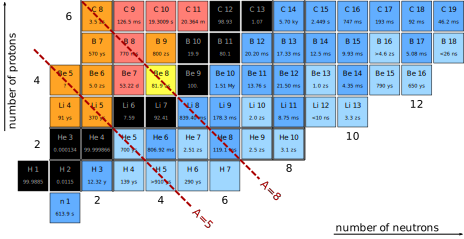
\includegraphics[width=0.85\textwidth]{graphics/bbn/chart_nuclides_bbn}
    \caption{The low-mass section of the chart of the nuclides with red, dashed lines indicating $A=5$ and $A=8$. These are the two mass regions that do not have any stable nuclides, thus effectively halting heavier element production in \ac{bbn}. Chart generated with a \href{https://github.com/kmiernik/Chart-of-nuclides-drawer}{python tool by Krzysztof Miernik}.}
    \label{fig:bbn:chart_nuclides_low_mass_region}
\end{figure}
Figure~\ref{fig:bbn:chart_nuclides_low_mass_region} shows an excerpt of the chart of the nuclides from hydrogen to carbon. Black isotopes are stable. The dashed, red lines indicate mass numbers $A=5$ and $A=8$, at which no stable nuclides exist. Thus, reactions of two \ex{4}He nuclei or a \ex{4}He nucleus and a proton do not form stable nuclides, which prevents \ac{bbn} from forming anything heavier than \ex{7}Li. 

While nucleosynthesis takes place, the universe continues expanding, thus the temperature further decreases. This significantly limits the time in which new nuclides can form. Below a temperature of $T_9\approx 0.1$ \ac{bbn} comes to a halt. This means that around 10-15\,min after the Big Bang, all the hydrogen, helium, and other \ac{bbn} products were formed. 

\begin{figure}[tb]
    \centering
    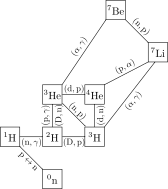
\includegraphics[width=0.4\textwidth]{graphics/bbn/reaction_network}
    \caption{\ac{bbn} reaction rate network for dominant reactions, after \citet{nollett2000}.}
    \label{fig:bbn:reaction_network}
\end{figure}
Figure~\ref{fig:bbn:reaction_network} shows the reaction network showing dominant reactions at work in \ac{bbn} \citep[after][]{nollett2000}. As is common, we abbreviate the \ex{4}He nucleus with the symbol $\alpha$. Reactions are written in their abbreviated form, as is common in nuclear physics. For example \ex{1}H(n,$\gamma$)\ex{2}H could also be written as \ex{1}H + n $\longrightarrow$ \ex{2}H + $\gamma$. Notably, there is no main reaction to produce \ex{6}Li. Lithium-7 can be produced in two ways: directly from tritium by capturing a $\alpha$ particle (which is equivalent to \ex{4}He capturing a tritium nucleus) or by production of \ex{7}Be (from \ex{3}He) and subsequent decay to \ex{7}Li.


\subsection{Observational Constraints}

So far, we have roughly derived the production of hydrogen and \ex{4}He expected to form during the Big Bang. We furthermore mentioned how D, \ex{3}He, and \ex{7}Li are produced. Our derivations were mainly based on the temperature and density evolution of the universe during \ac{bbn}, two quantities that are coupled to each other. By observing the abundances of hydrogen, helium, and lithium in the universe and deriving the fractions of the species of interest that formed in the Big Bang, we can constrain the environment in which \ac{bbn} took place. 

\begin{figure}[tb]
    \centering
    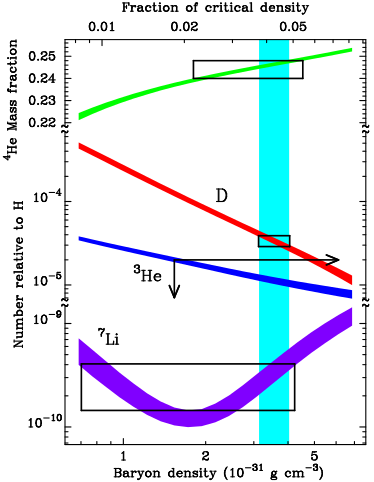
\includegraphics[width=0.5\textwidth]{graphics/bbn/tytler2000_fig2}
    \caption{\ac{bbn} predictions of the D, \ex{3}He, \ex{4}He, and \ex{7}Li abundance as a function of the present-day baryon density \citep{tytler20}. From \href{https://arxiv.org/abs/astro-ph/0001318}{\texttt{arXiv:astro-ph/0001318}}.}
    \label{fig:bbn:nuclides_baryon_density}
\end{figure}
Figure~\ref{fig:bbn:nuclides_baryon_density} shows the calculated abundances of D, \ex{3}He, \ex{4}He, and \ex{7}Li when varying the present-day baryon density. The squares show the observed ratios, where available, and their uncertainties. The larger the baryon density in the universe, the larger is the baryon-to-photon ratio. As discussed before, this ratio and the temperature define when deuterium can form (see Figure~\ref{fig:bbn:planck_radiation_deuterium_fusion}). If the baryon-to-photon ratio goes up, fewer neutrons decay until they are captured and thus more \ex{4}He nuclei are ultimately formed. The conversion of D to \ex{4}He will also be more complete, thus less deuterium remains. The higher starting abundance of D and higher end abundance of \ex{4}He also results in burning out \ex{3}He more effectively, thus lowering its abundance with an increase in the baryon density. The curve in Figure~\ref{fig:bbn:nuclides_baryon_density} for \ex{7}Li shows the competition of two reactions. At low baryon densities, \ex{7}Li is mainly produced via \ex{4}He + T $\longrightarrow$ \ex{7}Li + $\nu$. At increased baryon density, \ex{7}Li however gets again efficiently destroyed by burning further. This destruction is compensated and overtaken at even higher baryon densities since \ex{7}Be is produced more efficiently, which then immediately decays to \ex{7}Li.

While difficult to observe, the abundance of \ac{bbn}-produced hydrogen, helium, and lithium in the universe is a great way to determine crucial parameters of the Big Bang model. Similar insights can however also be gained by analyzing the \ac{cmb}.

\section{Recombination}

In Section~\ref{sec:bbn:standard_model:assumptions} we laid out the assumptions of the standard model of cosmology, one of which is that the overall charge in the universe is zero. During \ac{bbn}, the temperature too high to for electrons and nuclei to combine in order to produce a neutral gas. These components thus rather occur as a plasma. In order to create a neutral gas, the temperature has to sink to below $3000$\,K. At this temperature, the electrons combine with the atomic nuclei. Historically, this phase has been described as recombination, although the ``re'' part is slightly misleading since electrons and nuclei have never been combined previously.

During the plasma phase, i.e., prior to recombination, photons can scatter easily and the universe is thus opaque. After recombination the universe becomes transparent, and we transition into the matter dominated universe (see Figure~\ref{fig:bbn:cosmology_phases}). Since the Big Bang, roughly $4\times10^{5}$\,a have elapsed at this point.

The transition from the radiation dominated to the matter dominated universe can still be seen today as the horizon of the visible universe. It has significantly cooled down and is today seen as the \ac{cmb}. An image of is fluctuations is shown in Figure~\ref{fig:bbn:wmap_cmb}.


\section{Reading}

Since \ac{bbn} took place fairly long ago at this point, it seems adequate to also look at the literature from a historic point of view. For the historical perspective one should read \citet{alpher48} and \citet{peebles66prl}. These are both fairly short manuscripts. The present status of \ac{bbn} was recently given by \citet{cyburt16}. While this work contains fairly detailed methods on uncertainty calculations that are outside the scope of this lecture, please read sections III. Observations and V. The Lithium Problem in detail. You might also want to skim the introduction and the preliminaries.

For these readings it is important that you do not get hung up on details you do not understand, but rather try to follow the big picture. The following questions that can be discussed in class might help to focus on the big picture.

\begin{itemize}
    \item What elements and isotopes are all formed in the Big Bang according to the work by \citet{alpher48}? What are the issues you see with this model, especially regarding it from the current state of knowledge?
    \item What nuclides were produced in the Big Bang according to \citet{peebles66prl} and how does this differ from the work by \citet{alpher48}?
    \item Note the neutron half-life that is used in \citet{peebles66prl}. What is the issue here? This is also in detail discussed in the introduction by \citet{cyburt16}.
    \item What importance does the nuclear reaction rate network have in \citet{cyburt16}? What reaction rates are to this day fairly uncertain?
    \item Discuss how the primordial abundance of H, D, \ex{3}He, \ex{4}He, and \ex{7}Li can be derived from current observations. What are the problems?
    \item What is meant in \citet{cyburt16} by ``regression to zero metallicity''?
\end{itemize}